\documentclass[a4paper,BCOR7mm,12pt,pointlessnumbers,bibtotoc]{scrartcl}

\usepackage{amsmath,epsfig}
\usepackage{amssymb,amsfonts}
\usepackage{color}
\usepackage{array,booktabs}
\usepackage{graphicx}
\usepackage{caption}
\usepackage[hypcap=true,labelformat=simple]{subcaption}
\renewcommand{\thesubfigure}{(\alph{subfigure})}
\usepackage{tikz}
\usetikzlibrary{arrows,automata}
\usepackage{listings}
\usepackage{hyperref}
\usepackage{enumitem}

\newcolumntype{C}[1]{>{\centering\arraybackslash}p{#1}} % centering column type with fixed width
\newcolumntype{R}[1]{>{\raggedleft\arraybackslash}p{#1}} % right aligned column type with fixed width
\newcolumntype{L}[1]{>{\raggedright\arraybackslash}p{#1}} % left aligned column type with fixed width

\newcommand{\ceil}[1]{\left\lceil #1 \right\rceil} %\left\lceil #1 \right\rceil

\begin{document}
%\maketitle
\begin{center}
\Large Ternary Adder IP Cores\\[0.4cm]
\large Martin Kumm, Jens Willkomm \\[0.5cm]
\large \today \\[0.5cm]
\end{center}

\section{Introduction}

This IP core provides resource efficient ternary adders, i.\,e., adders with three inputs performing $s = x + y + z$, for the Altera and Xilinx platforms. 
Resource efficient means that they need exactly the same resources on modern FPGAs as two-input adders, but are slightly slower.
The Xilinx core (\verb|ternary_adder_xilinx.vhd|) is a low-level implementation, following an US patent from Xilinx \cite{sp07}. It directly uses the Xilinx primitives (\verb|CARRY4|, \verb|LUT6_2| and \verb|FDCE|). It is suitable for all FPGAs providing 6-input LUTs. Today, these are the Virtex~5-7, Spartan~6, Kintex~7 and Artix~7 families. The Altera core (\verb|ternary_adder_altera.vhd|) is a high-level implementation using the '+' operator. However, the ternary subtract operations ($x - y + z$, $x + y - z$ and $x - y - z$) are not supported by a high-level description; so this is realized by extending the word size of the ternary adders and setting the lower bits to appropriate constant values. 
They can be mapped very resource efficient for all Altera FPGAs providing adaptive logic modules (ALMs), today, these are the Arria I,II,V and Stratix II-V FPGAs.

\section{Interface}

The generics as well as the port are identical for the Altera and Xilinx implementation and are described in Table~\ref{tab:generics} and Table~\ref{tab:port}, respectively.

\begin{table}[!h]
	\renewcommand{\arraystretch}{1.1}
	\caption{Description of the generics}
	\label{tab:generics}
	\centering
	\begin{tabular}{lccL{7cm}}
	  \toprule
	  Generic & Type & Default & Description\\
    \cmidrule(rl){1-1} \cmidrule(rl){2-2} \cmidrule(rl){3-3} \cmidrule(rl){4-4}
    \verb|input_word_size|  & integer & 10    & Input word size of the inputs $x$,$y$ and $z$. The output word size is automatically set to \verb|input_word_size+2|\\
    \verb|subtract_y|       & boolean & false & Input $y$ is negated, realizing $s = x - y \pm z$\\
    \verb|subtract_z|       & boolean & false & Input $z$ is negated, realizing $s = x \pm y - z$\\
    \verb|use_output_ff|    & boolean & true  & If true, the adder uses flip flops at the output (without extra slice or ALM resources)\\
    \bottomrule
   \end{tabular}
\end{table}

\begin{table}[!h]
	\renewcommand{\arraystretch}{1.1}
	\caption{Description of the port}
	\label{tab:port}
	\centering
	\begin{tabular}{lcccL{5cm}}
	  \toprule
	  Generic & Direction & Type & Word Size & Description\\
    \cmidrule(rl){1-1} \cmidrule(rl){2-2} \cmidrule(rl){3-3} \cmidrule(rl){4-4} \cmidrule(rl){5-5}
    \verb|clk_i| & in  & \verb|sl|        & 1                    & Clock input (used when \verb|use_output_ff=true|)\\
    \verb|rst_i| & in  & \verb|sl|        & 1                    & Reset input (used when \verb|use_output_ff=true|)\\
    \verb|x_i|   & in  & \verb|slv| & \verb|input_word_size|     & Input $x$\\
    \verb|y_i|   & in  & \verb|slv| & \verb|input_word_size|     & Input $y$\\
    \verb|z_i|   & in  & \verb|slv| & \verb|input_word_size|     & Input $z$\\
    \verb|sum_o| & out & \verb|slv| & \verb|input_word_size + 2| & Sum output $s$\\
    \bottomrule
   \end{tabular}
\end{table}

\section{Implementation}

Both implementations uses a carry save adder (CSA) tree with three inputs and a final ripple carry adder as vector merging adder (VMA). One stage of full adders (FAs) is used to realize a 3:2 compressor, i.\,e., the three input bit vectors are compressed to two bit vectors which are obtained by the sum and carry outputs. A second stage of FAs merges these two bit vectors to a single result.

For Altera, the 3:2 compressor can be directly mapped to the ALM LUT, realizing the sum $s'_i = x_i \oplus y_i \oplus z_i$ and carry $c'_i = x_i y_i + x_i z_i + y_i z_i$. The full adders of the ALM are used for the VMA. 
To include both stages in a single ALM stage, each ALM has to be configured to the shared arithmetic mode \cite{blsy09} in which the output of one LUT is connected to the FA input of the next higher bit. The resulting ternary adder structure is shown in \figurename~\ref{fig:ternary_adder_stratix}. 

For Xilinx, the FA for the 3:2 compressor is also realized in the FPGA LUT \cite{sp07}. In addition to that, one additional XOR gate has to be realized in the same LUT to complete the fast carry chain resources to a ripple carry adder for the VMA. The carry output of the first FA (realized in the LUT) must be routed to the next higher FA input using the FPGA routing fabric.
The resulting slice configuration is shown in \figurename~\ref{fig:ternary_adder_virtex_5_6_7}.


\begin{figure}[!h]
\centering
% \subfigure[]{\scalebox{1}{\includegraphics{images/ternary_adder_generic}\label{fig:ternary_adder_generic}}}
% \subfigure[]{\scalebox{1}{\includegraphics{images/ternary_adder_3_2_comp}\label{fig:ternary_adder_3_2_comp}}}
	\begin{subfigure}[c]{\columnwidth}
	  \centering
    \scalebox{1.2}{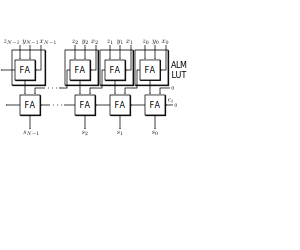
\includegraphics{images/ternary_adder_altera}}
		\caption{}
		\label{fig:ternary_adder_stratix}
	\end{subfigure}
	\begin{subfigure}[c]{\columnwidth}
	  \centering
    \scalebox{1.2}{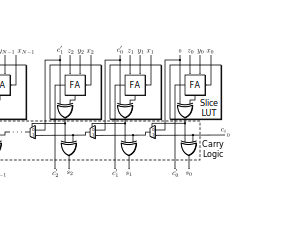
\includegraphics{images/ternary_adder_xilinx}}
		\caption{}
		\label{fig:ternary_adder_virtex_5_6_7}
	\end{subfigure}
 \caption{Realization of ternary adders 
 %(a) generic architecture using two ripple carry adders 
 on
 (a) Altera Stratix II-V ALMs (b) Xilinx Virtex 5-7 Slices}
 \label{fig:ternary_adders}
\end{figure}

\section{Resource Consumption}

For Altera, each ALM can compute two output bits. As the output word size is two bits more than the input word size, there are 
\begin{align}
	N_{\text{ALM},++} = \ceil{\frac{\text{input\_word\_size}+2}{2}} 
\end{align}
ALMs needed for a pure addition ($s = x + y + z$). If one input is subtracted (setting one of \verb|subtract_y| or \verb|subtract_y| to true), the word length has to be extended by one bit leading to:
\begin{align}
	N_{\text{ALM},+-} = \ceil{\frac{\text{input\_word\_size}+3}{2}}
\end{align}
Finally, if two inputs are subtracted, the word length has to be further increased leading to:
\begin{align}
	N_{\text{ALM},--} = \ceil{\frac{\text{input\_word\_size}+4}{2}} 
\end{align}

For Xilinx, four output bits can be computed in each slice. Thus, the number of slices is given by:
\begin{align}
	N_{\text{Slices}} = \ceil{\frac{\text{input\_word\_size}+2}{4}} 
\end{align}
The slice usage is independent of the operation performed. If a slice is not fully utilized, the remaining LUTs can still be used for other functionallities.

\section{Performance}

To estimate the performance, the maximum clock frequencies ($f_\text{max}$) were obtained by synthesis experiments for Altera Stratix~IV (EP4SGX230KF40C2) using Quartus-II~10.1 and Xilinx Virtex~6 (XC6VLX75T-2FF484) using ISE 13.4, both after place \& route. The resulting clock frequencies with output word sizes from 16 up to 64\,bit are shown in Table~\ref{tab:performance}.

\begin{table}[!h]
	\renewcommand{\arraystretch}{1.1}
	\caption{Performance of the IP Cores}
	\label{tab:performance}
	\centering
	\begin{tabular}{ccc}
	  \toprule
      output word size & $f_\text{max}$ Stratix IV [MHz] & $f_\text{max}$ Virtex 6 [MHz]\\
	    \cmidrule(rl){1-1} \cmidrule(rl){2-2} \cmidrule(rl){3-3}
      16 & 708 & 450\\
      32 & 565 & 379\\
      48 & 479 & 312 \\
      64 & 423 & 292\\
    \bottomrule
   \end{tabular}
\end{table}

\section{Simulation \& Test}

The simulation and automated tests were performed using Modelsim. For that, a testbench (\verb|tb_ternary_adder.vhd|) was created which uses a random number generator together with assert statements to verify the designs. To automate the different FPGA targets the do-file \verb|batch_sim.do| was created which compiles the designs and applies the tests for each target as specified in the do-file \verb|sim_single_inst.do|. These tests include different word sizes, subtractions and the output flip flop functionality. All tests can be started from command line using \verb|vsim -c -do 'do batch_sim.do'| (as defined in \verb|modelsim_batch_sim.sh|).

\bibliographystyle{alpha}
\bibliography{ternary_adder}

\end{document}


 
